% Appendix J: Bayesian inference for the coupling-space survey.
% Six paragraphs covering: opening + amplification score + evidence
% integral + cubed-sphere joint prior + evidence as prior expectation
% + posterior contraction.  PolyChord and per-scalar prior families
% are deliberately not given their own paragraphs (the cubed-sphere
% is the project's prior architecture; PolyChord is cited in the
% opening only).

\section{Bayesian inference architecture}%
\label{InferenceArchitecture}

The inference layer producing the survey results of
\cref{Results} explores the high-dimensional PGT+EM coupling space
catalogued in \cref{PGTEnumeration}, where many equivalent
parametrisations of the same physics appear in the
literature~\cite{barker2024poincare,lin2019pgt,karananas2014parity,blagojevic2018hamiltonian,bahamonde2025cubic}
and individual coefficient values are conventional labels for
combinations of underlying interactions.  We use
PolyChord~\cite{Handley:2015fda,Handley:2015vkr,Skilling:2004pqw,Ashton:2022grj}
for the nested sampling, with anesthetic~\cite{Handley:2019mfs} for
the posterior visualisation as corner plots and as per-tile panel
maps over the atlas of \cref{CubedSphereAtlas}.  From the sampler we
obtain the prior-averaged amplification $\mathcal{Z}$
(\cref{EvidenceIntegral}) and the Kullback--Leibler divergence
$D_{\mathrm{KL}}$~\cite{Kullback:1951zyt,Handley:2019mfs}, which
captures how concentrated the score-weighted posterior is on a
particular region of coupling space.  The survey then reports which
regions activate the Gertsenshtein amplification, and which
invariant combinations they encode.

\paragraph*{Amplification score}
The PDE solver~(\cref{NumericalEvolution}) evolves the linearised
perturbations for an integration time $t_\mathrm{end}$ and returns
the exit conversion probability $P(\theta, t_\mathrm{end})$ at each
coupling vector $\theta$ (the parametrisation of
\cref{PGTEnumeration}).  The score function for the nested sampler
is the amplification of this exit value over its Einstein--Maxwell
baseline~\cref{GertsenshteinFormula},
\begin{equation}
  A(\theta) \;=\; \frac{P(\theta, t_\mathrm{end})}{\sin^2(\kappa\Bzero t_\mathrm{end}/2)},
  \label{AmplificationScore}
\end{equation}
with the baseline shown for the uniform-magnetic-background setup
of \cref{Results}; for a localised-$\Bzero$ configuration the
baseline becomes the path-integrated form
\cref{BoccalettiPathIntegrated}, with the surrounding analysis
otherwise unchanged.\footnote{$A(\theta)$ and the asymptotic
survey-coefficient ratio $\Aamp$ of \cref{AmplificationFactor} are
different objects: $A(\theta)$ is the actual finite-time exit ratio
at the simulation's $t_\mathrm{end}$, while $\Aamp$ is the
leading-order Taylor coefficient extracted in the small-$\kappa\Bzero
t$ limit.  The two agree to leading order whenever the integrated
$A$ stays close to its short-time linear growth --- as in the
uniform-background, perturbative-$\Pmax$ regime of this work --- and
diverge whenever the wave has time to accumulate non-leading-order
behaviour, as can happen once the localised-$\Bzero$ extensions
introduce a finite interaction-region traversal time.}  The
nested-sampling likelihood is
\begin{equation}
  \log L(\theta) \;=\; \pm\log A(\theta),
  \label{NestedScore}
\end{equation}
with the sign chosen to direct the survey toward amplifying ($+$)
or suppressing ($-$) regions of coupling space.


\begin{figure}[t]
  \centering
  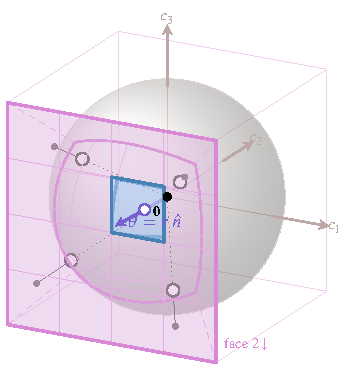
\includegraphics[width=\linewidth]{figures/cubed_sphere_atlas.pdf}
  \caption{Gnomonic cubed-sphere atlas used to sample the direction
    $\hat n \in S^{N-1}$ of a joint coupling-space prior, drawn for
    $N=3$.  Axes $c_1, c_2, c_3$ are the coupling-space coordinates.
    The semi-transparent grey sphere is $S^{N-1}$; an $N$-cube is
    wrapped around the origin (blue wireframe) and each cube face is
    radially projected onto the sphere.  The highlighted face
    (face~$2\!\downarrow$, transparent blue) is one \emph{cube-tile} of
    the atlas, partitioned into $4\times 4$ sub-tiles whose
    constrained-prior chains run independently; the curves on the
    sphere bound the \emph{sphere-tile} --- the gnomonic image of the
    cube-tile --- and the projected gridlines within it carry the
    sub-tile partition onto the curved surface, with one sphere
    sub-tile highlighted in blue to match its cube-face pre-image.
    Dotted lines from the origin through cube-tile anchor points are
    gnomonic projection rays; the small ring markers show where each
    ray meets the sphere.  The green arrow is one sample vector
    $\theta = r\,\hat n$ through the highlighted sub-tile: the dark
    segment inside the cube and the arrow segment emerging past the
    face show the two-step decomposition of the radial-direction
    prior into a magnitude $r$ and a direction $\hat n$, with the
    filled disc marking where the vector pierces the face and the
    ring marker where it crosses $S^{N-1}$.  The figure idiom
    follows~\cite{chen2021lmars}.}
  \label{CubedSphereAtlas}
\end{figure}

\paragraph*{Cubed-sphere joint prior}
The natural objects of the survey are the directions in the invariant
space rather than the values of any individual coefficient, so we
decompose a coupling vector $\theta \in \mathbb{R}^N$ as
$\theta = r\,\hat n$, with $r>0$ the overall
perturbation magnitude away from the Einstein--Maxwell baseline and
$\hat n \in S^{N-1}$ the direction in the
parametrisation of \cref{PGTEnumeration}.  The survey question
becomes which direction $\hat n$ at fixed $r$
activates the Gertsenshtein amplification.  We sample $\hat n$
uniformly on
$S^{N-1}$ via a gnomonic cubed-sphere atlas: the $N$-cube wrapped
around the origin is radially projected onto $S^{N-1}$, yielding a
quasi-rectilinear angular grid without polar
singularities~(\cref{CubedSphereAtlas}).  Each face partitions
further into sub-tiles whose constrained-prior chains run
independently and are pooled into the joint $\hat n$
distribution at the end.  In the limit of fine sub-tile resolution
each tile becomes locally rectilinear and the chart approaches a
flat Cartesian one on the sphere, so the construction interpolates
smoothly between a coarse global parametrisation of $S^{N-1}$ and
the local-flat limit familiar from Cartesian coupling-space
sampling.\footnote{The atlas used here is adapted from
W.~E.~V.~Barker's unreleased extension of the \textsc{psalter}
package~\cite{barker2024psalter,barker2025psalter2}, shared with this
project for implementation guidance.  The underlying gnomonic
projection is the standard cubed-sphere construction
of~\cite{ronchi1996cubedsphere}.}

\paragraph*{Bayesian evidence}
With $L(\theta) = A(\theta)$ from \cref{NestedScore}, the Bayesian
evidence targeted by the nested sampler is a prior expectation over
the amplification score,
\begin{equation}
  \mathcal{Z} \;=\; \int A(\theta)\,\pi(\theta)\,\diff\theta
  \;=\; \langle A\rangle_\pi,
  \label{EvidenceIntegral}
\end{equation}
the average amplification of the Gertsenshtein conversion over the
coupling prior.  A theory with $\log\mathcal{Z}\approx 0$ offers no
amplification on average across the prior; a theory with
$\log\mathcal{Z}\gg 0$ has typical coupling vectors that amplify the
conversion above its Einstein--Maxwell baseline; one with
$\log\mathcal{Z}\ll 0$ has $\langle A\rangle_\pi \ll 1$.  The
absolute value of $\mathcal{Z}$ is controlled by the choice of prior
support and is not the load-bearing output of the survey; what we
report from $\mathcal{Z}$ is the sign and order of magnitude of
$\log\mathcal{Z}$, with the corresponding structural information
carried jointly by $D_{\mathrm{KL}}$, introduced next.

\paragraph*{Posterior contraction}
Nested sampling produces samples from the score-reweighted posterior
\begin{equation}
  p(\theta\mid A) \;\propto\; A(\theta)\,\pi(\theta),
  \label{ScorePosterior}
\end{equation}
the reweighting of the prior by the amplification score.  Its
information content relative to the prior is the Kullback--Leibler
divergence
\begin{equation}
  D_{\mathrm{KL}}\big(p(\theta\mid A)\,\|\,\pi(\theta)\big)
  \;=\; \int p(\theta\mid A)\,
  \log\!\frac{p(\theta\mid A)}{\pi(\theta)}\,\diff\theta,
  \label{KLDivergence}
\end{equation}
measured in nats.  Small $D_{\mathrm{KL}}$ means the posterior is
indistinguishable from the prior and the response is generic to the
theory across the surveyed range; large $D_{\mathrm{KL}}$ means the
posterior has contracted onto a specific coupling region and the
response is parameter-specific.  $D_{\mathrm{KL}}$ depends only on the contraction of the prior into
the posterior, not on the absolute prior volume that scales
$\mathcal{Z}$.  When $D_{\mathrm{KL}}$ is large at small
$\mathcal{Z}$ the theory is generically non-amplifying over the
surveyed prior while a small region of coupling space \emph{is}
amplifying and the chain has contracted onto it.  The per-coupling
marginal $D_{\mathrm{KL}}$ extracted with
anesthetic~\cite{Handley:2019mfs} then picks out which invariants
the chain has contracted along, telling us not just \emph{that} a
region of coupling space carries the response but \emph{which
directions in operator space} it spans.  Campaign values for
$\mathcal{Z}$, $D_{\mathrm{KL}}$, and the marginal
$D_{\mathrm{KL}}$ are reported in \cref{Results}.
